
\begin{center}
    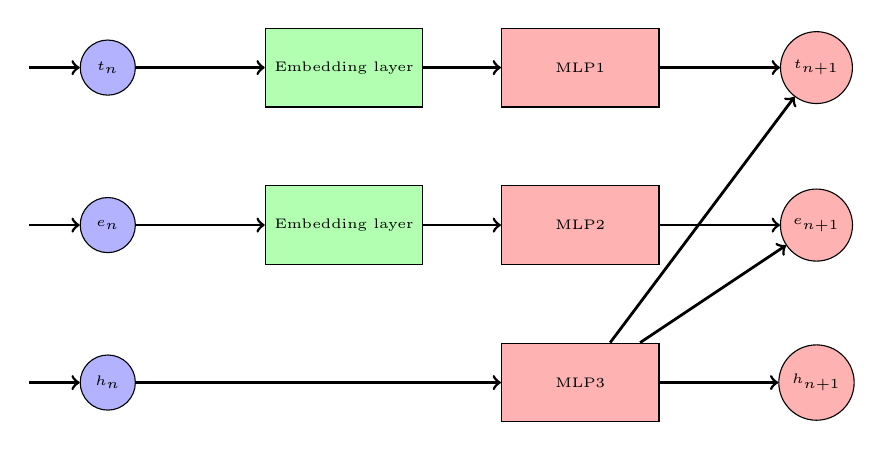
\begin{tikzpicture}[
            neuron/.style={circle, draw, minimum size=0.7cm},
            rect neuron/.style={rectangle, draw, minimum width=2cm, minimum height=1cm}, % Rectangular neuron
            input neuron/.style={neuron, fill=blue!30},
            embeddings neuron/.style={rect neuron, fill=green!30},
            mlp neuron/.style={rect neuron, fill=red!30},
            output neuron/.style={neuron, fill=red!30},
            every node/.style={align=center,font=\tiny}
        ]
        % Input layer
        \node[input neuron] (I1) at (0,2) {$t_n$};
        \node[input neuron] (I2) at (0,0) {$e_n$};
        \node[input neuron] (I3) at (0,-2) {$h_{n}$};
        % Hidden layer
        \node[embeddings neuron] (H1) at (3,2) {Embedding layer};
        \node[embeddings neuron] (H2) at (3,0) {Embedding layer};
        
        \node[mlp neuron] (MLP1) at (6,2) {MLP1};
        \node[mlp neuron] (MLP2) at (6,0) {MLP2};
        \node[mlp neuron] (MLP3) at (6,-2) {MLP3};
        % Output layer
        \node[output neuron] (O1) at (9,2) {$t_{n+1}$};
        \node[output neuron] (O2) at (9,0) {$e_{n+1}$};
        \node[output neuron] (O3) at (9,-2) {$h_{n+1}$};

        % Connections
        \draw[->,line width=1px] (I1) -- (H1);
        \draw[->,line width=1px] (I2) -- (H2);
        \draw[->,line width=1px] (-1,2) -- (I1);
        \draw[->,line width=1px] (-1,0) -- (I2);
        \draw[->,line width=1px] (-1,-2) -- (I3);
        
        \draw[->,line width=1px] (H1) -- (MLP1);
        \draw[->,line width=1px] (H2) -- (MLP2);
        \draw[->,line width=1px] (I3) -- (MLP3);
        
        \draw[->,line width=1px] (MLP1) -- (O1);
        \draw[->,line width=1px] (MLP2) -- (O2);

        \draw[->,line width=1px] (MLP3) -- (O1);
        \draw[->,line width=1px] (MLP3) -- (O2);
        \draw[->,line width=1px] (MLP3) -- (O3);

    \end{tikzpicture}
  \end{center}
